\documentclass[12 pt, a4paper]{article}

\usepackage[utf8]{inputenc}
\usepackage[brazil]{babel}
\usepackage[top=3cm, bottom=2cm, left=3cm, right=2cm]{geometry}
\usepackage{graphicx}
\usepackage{indentfirst}
\usepackage{enumerate}
\usepackage{amsmath, amsfonts, amssymb}
\usepackage{float}

\usepackage{listings}
\usepackage{color}
\renewcommand\lstlistingname{Quelltext} % Change language of section name

\lstset{ % General setup for the package
	%frame=tb,
	language=C, % choose the language of the code
	basicstyle=\small\sffamily, % the size of the fonts used for the code
	numbers=left, % where to put the line-numbers
	numberstyle=\tiny, % size of the fonts used for the line-numbers
	stepnumber=2, % the step between two line-numbers.
	numbersep=5pt, % how far the line-numbers are from the code
	backgroundcolor=\color{white}, % sets background color (needs package)
	showspaces=false, % show spaces adding particular underscores
	showstringspaces=false, % underline spaces within strings
	showtabs=false, % show tabs within strings through particular underscores
	frame=none, % adds a frame around the code
	columns=fixed, 
	keepspaces,
	commentstyle=\color{red},
	keywordstyle=\color{blue}
	tabsize=4, % sets default tab-size to 2 spaces
	captionpos=b, % sets the caption-position to bottom
	breaklines=true, % sets automatic line breaking
	breakatwhitespace=false, % automatic breaks happen at whitespace
	morecomment=[l]{//} % displays comments in italics (language dependent)
}


\begin{document}

	\begin{titlepage}
		\begin{center}
			{\large \textbf{Universidade de Bras\'ilia}}\\
			{\large \textbf{Departamento de Ci\^encia da Computa\c{c}\~ao}}\vspace{1.0cm}

			{\Huge \textbf{\'Arvores bin\'arias}}\\[7.0cm]
			
\includegraphics[height=10em]{images/CIC_header}\\[6.0cm]

		\end{center}

		\begin{table}[h]
		\begin{tabular}{l l}
		Aluno:    	& Hiago dos Santos Rabelo\\
		Disciplina:	& Estrutura de dados\\
		Professor:	& Eduardo A. P. Alchieri\vspace{1.5cm}\\

		\end{tabular}
		\end{table}


		\center \date[Novembro de 2017
			
	\end{titlepage}

\tableofcontents

\newpage
\section {Introdu\c{c}\~ao}

O problema a ser resolvido consiste em se ler um arquivo .txt e armazenar suas informa\c{c}\~oes tanto em uma \'arvore bin\'aria de busca como em uma lista, posteriormente usar essa informa\c{c}\~ao para decodificar uma mensagem codificada em morse. 
\newline
Por fim, mostrar a diferen\c{c}a entre o tempo de decodifica\c{c}\~ao usando-se listas e usando-se \'arvores bin\'arias de busca.

\newpage
\section {Implementa\c{c}\~ao}

\subsection{Estrutura de dados utilizada}

As estruturas de dados utilizadas para resolver o problema proposto no trabalho foram: \'arvore bin\'aria de busca e listas. 

\begin{enumerate}[(i)]
	\item \'Arvore bin\'aria de busca:
	\begin{itemize}
	\item[-] Tem por fun\c{c}\~ao armazenar os caracteres na ordem de seus respectivos c\'odigos em morse, sendo que isso \'e feito de forma que quando o caractere \'e inserido na \'arvore \'e lido caractere por caractere de seu c\'odigo morse e para cada simbolo lido \'e tomado um caminho diferente. 
    

    Tomando-se o exemplo do caractere \texttt{A} codificado como: \texttt{.-.}
    \newline
    Logo, temos que acessar o filho da esquerda, depois o da direita e depois o da esquerda, sendo que como chegou ao fim do c\'odigo especificado devemos colocar o caractere \texttt{A} nesse n\'o. Seguindo-se esse mesmo racioc\'inio para o restante dos caracteres.
    \begin{figure}[H]
        \centering
        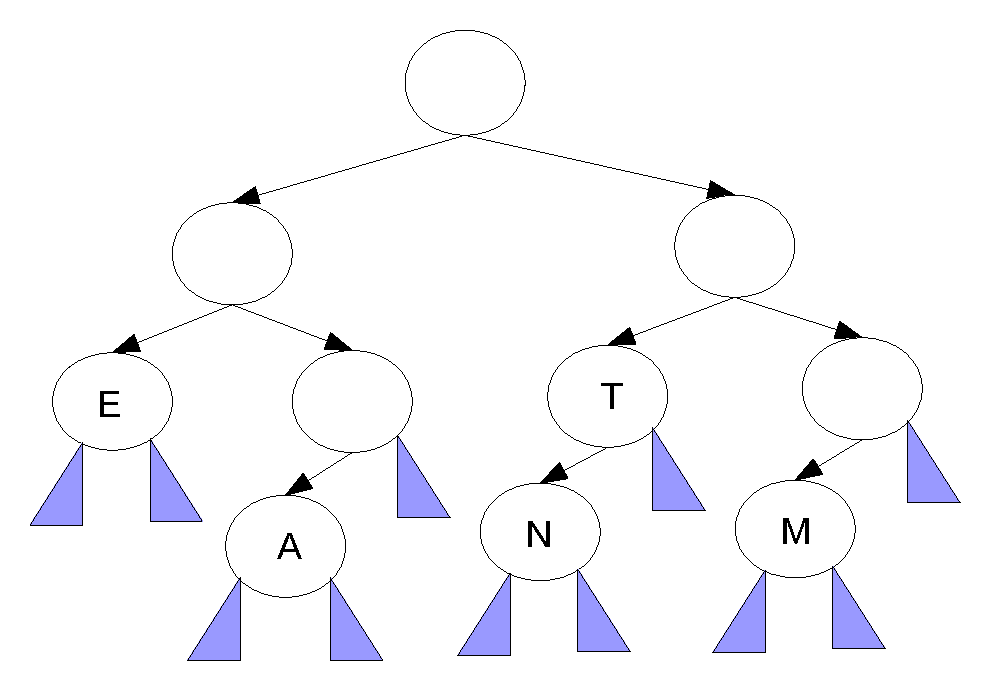
\includegraphics[scale = 0.4]{images/arvore}
        \caption{\'Arvore com chave do código morse}
        \label{arvore}
    \end{figure}
	\end{itemize}

	\item Lista :
	\begin{itemize}
	   \item[-] Tem por fun\c{c}\~ao armazenar os caracteres, seus respectivos c\'odigos em morse e um ponteiro para o pr\'oximo elemento, sendo que ponteiro do \'ultimo elemento aponta para NULL. 
       \newline
       Sendo assim, quando for feita a busca para tentar descriptografar a mensagem dever\'a ser percorrida a lista desde o in\'icio at\'e que se seja encontrado o c\'odigo o qual se est\'a  buscando e assim extrair o caractere que corresponde a esse caractere e que se encontra armazenado na mesma posi\c{c}\~ao da lista em que se estava o caractere correspondente.\\

        \begin{figure}[H]
        \centering
        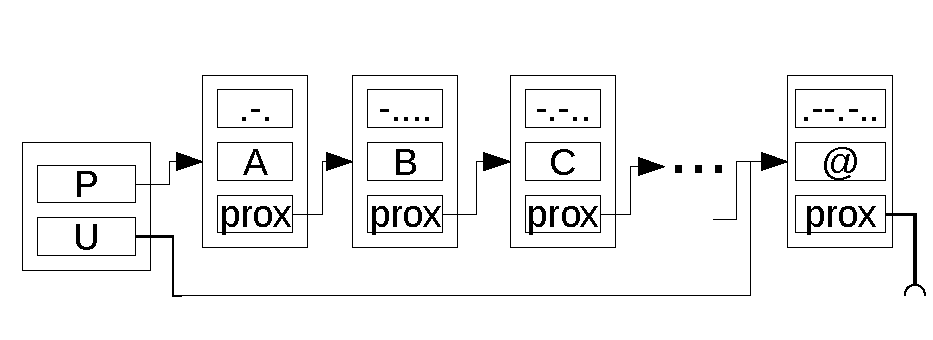
\includegraphics[scale = 0.52]{images/lista}
        \caption{Lista float.}
        \label{lista}
        \end{figure}
    \end{itemize}
\end{enumerate}

\subsection{Principais fun\c{c}\~oes}

Temos a seguir os nomes das principais funções, iguais aos colocados no programa, e suas respectivas descrições:
\begin{enumerate}[(i)]
    \item cria\_no :
        \begin{itemize}
            \item[-] Aloca espaço de memória para a estrutura do tipo \textit{no} então retornando o endereço do espaço alocado e caso não seja possível retorna NULL, sendo que irá colocar NULL na variável prox dentro da estrutura alocada.
        \end{itemize}
    \item passa\_arquivo\_chave\_para\_arvore:
        \begin{itemize}
            \item[-] recebe como par\^ametro o nome do arquivo com a codifica\c{c}\~ao morse e lendo desse arquivo, caso exista e possa ser lido, as codifica\c{c}\~oes e seus respectivos caracteres. Sendo que essa informa\c{c}\~ao \'e passada para a \'arvore como descrito acima.
        \end{itemize}
    \item zera\_lista:
        \begin{itemize}
        \item[-] recebe como par\^ametro uma lista e atribui ao ponteiro do primeiro elemento e do \'ultimo o valor NULL.'
        \end{itemize}
    \item decodifica\_usando\_arvore:
        \begin{itemize}
            \item[-] recebe como par\^ametro o nome do arquivo com a mensagem para ser decodificada e usando a \'arvore bin\'aria de busca para decodificar. Sendo que, l\^e simbolo por s\'imbolo e percore a \'arvore para achar o caractere correspondente usando a rela\c{c}\~ao de caso o simbolo seja '\textit{.}' dever\'a ir para o filho da esquerda e caso seja '\textit{-}' ent\~ao dever\'a ir para o filho da direita.
        \end{itemize}
    \item decodifica\_usando\_lista:
        \begin{itemize}
            \item[-] Recebe como parâmetros o endereço da lista de elementos (cada elemento contendo um código e seu respectivo caractere como mostrado na Figura \ref{lista}) e o nome do arquivo a ser decodificada e percorre uma busca na lista para achar o caractere desejado.
        \end{itemize}
\end{enumerate}

\newpage
\section {Conclus\~ao}
	Conclui-se que este trabalho requisitou v\'arios conhecimentos adiquiridos na mat\'eria de Algoritmos e Programa\c{c}\~ao de Computadores, tendo como principais dificuldades o armazenamento e leitura da lista.



    Por fim, foi poss\'ivel notar que o programa, que utilizava o algoritmo de \'arvore bin\'aria de busca, para resolver o problema foi consideravelemente mais r\'apido do que o programa que utilizava lista, uma vez que a seguinte opera\c{c}\~ao 

	\begin{lstlisting}
	tempo_medido = clock() - tempo_medido;
	\end{lstlisting}

	resultou em  0.000031 segundos sendo utilizada a \'arvore e 0.000066 segundos sendo utilizada a lista.

\newpage
\addcontentsline{toc}{section}{Refer\^encias}

\bibliographystyle{ieeetr}
\bibliography{mybib}

\nocite{*}
%\cite{luis,tex,Cecilia,bibl}


\end{document}
